\chapter{군속도, 페르미온의 배타 원리, 디랙 바다}

\section{위상 속도와 군속도}

\begin{classroomqa}
\lecturetimestamp{00:00:07}
\audiencequestion{군속도와 위상 속도란 무엇인가요?}
\lecturerresponse{위상 속도는 평면파에서 위상이 일정한 한 점을 따라간다. 일반적으로 측정 가능한 물체의 운동을 나타내지는 않는다. 군속도는 파동 묶음의 포락선을 따라가며, 입자·신호·확률 흐름과 관련된 속도다.}
\end{classroomqa}

평면파,
\begin{equation}
\psi(x,t)=e^{i(kx-\omega t)},
\end{equation}
또는 그 실수형에서 시작하자.
\begin{equation}
\psi(x,t)=\sin(kx-\omega t).
\end{equation}
마루나 골, 또는 위상이 일정한 다른 점은 다음 조건을 만족하며 움직인다.
\begin{equation}
kx-\omega t=\text{constant}.
\end{equation}
편의상 상수를 0으로 두면
\begin{equation}
x=\frac{\omega}{k}t,
\qquad
v_{\mathrm{phase}}=\frac{\omega}{k}.
\end{equation}
\(\omega=2\pi/T\)와 \(k=2\pi/\lambda\)이므로,
\begin{equation}
v_{\mathrm{phase}}=\frac{\omega}{k}=\frac{\lambda}{T}.
\end{equation}
이는 한 주기 동안 주어진 위상이 진행하는 거리일 뿐이다.

비상대론적 Schr\"odinger 파동에서 \(\hbar=1\)이면 에너지와 운동량은 각각 \(\omega\)와 \(k\)이므로,
\begin{equation}
\omega(k)=\frac{k^2}{2m}.
\end{equation}
따라서 위상 속도는
\begin{equation}
v_{\mathrm{phase}}=\frac{k}{2m}.
\end{equation}
이다. 그러나 운동량이 \(k\)인 입자의 보통의 속도는 \(k/m\)이다. 두 값이 두 배 차이 난다는 점은 평면파 위상의 이동이 입자의 운동을 나타내지 않는다는 첫 번째 경고다.

더욱 분명한 경고도 있다. 모든 진동수에 같은 상수 \(C\)를 더해 보자.
\begin{equation}
\omega(k)\longrightarrow \omega(k)+C.
\end{equation}
예를 들어 이 상수는 \(mc_{\mathrm{light}}^2\)처럼 공통된 정지 에너지 항을 나타낼 수 있지만, 그 구체적인 이름은 중요하지 않다. 여기서 \(C\)는 빛의 속도가 아니라 에너지 오프셋이다. 위상 속도는 다음과 같이 바뀐다.
\begin{equation}
v_{\mathrm{phase}}\longrightarrow
\frac{\omega(k)+C}{k}
=v_{\mathrm{phase}}+\frac{C}{k}.
\end{equation}
하지만 모든 에너지에 같은 상수를 더해도 에너지 차이는 변하지 않으므로 비상대론적 물리에는 아무 변화가 없다.

파동함수에서 이를 직접 확인할 수 있다. 일반적인 Schr\"odinger 장을 모드들의 합 또는 적분으로 쓰면
\begin{equation}
\psi(x,t)=\sum_k a_k e^{ikx}e^{-i\omega(k)t},
\end{equation}
정규화 인자는 생략했다. 에너지를 이동시키면
\begin{align}
\psi(x,t)
&\longrightarrow
\sum_k a_k e^{ikx}e^{-i[\omega(k)+C]t}
\\
&=e^{-iCt}\psi(x,t).
\end{align}
모든 모드에 시간에 따라 변하는 같은 위상 인자가 붙는다. 켤레 장에는 반대 위상 인자가 붙으므로
\begin{equation}
\begin{aligned}
\psi^*(x,t)\psi(x,t)
&\longrightarrow
e^{iCt}e^{-iCt}\psi^*(x,t)\psi(x,t)
\\
&=\psi^*(x,t)\psi(x,t).
\end{aligned}
\end{equation}
기댓값에서도 같은 상쇄가 일어난다. 에너지의 영점을 이동했을 때 값이 변하는 양은 Schr\"odinger 입자의 물리적인 전파 속도일 수 없다. 따라서 위상 속도는 관례에 따라 달라지는 측면이 있다.

국소화된 입자는 무한 평면파 하나가 아니라 파동 묶음으로 표현된다. 구성 파동들은 파동 묶음이 있는 영역에서는 보강 간섭을 일으키고, 그 바깥에서는 상쇄 간섭을 일으킨다. 이 무늬의 운동은 서로 가까운 두 파동만으로도 구할 수 있다:
\begin{equation}
\psi(x,t)=
\sin(kx-\omega t)+
\sin(k'x-\omega't),
\end{equation}
여기서 \(k'\)는 \(k\)에 가깝고 \(\omega'=\omega(k')\)이다. 두 파동의 위상이 일치하는 곳에서 보강 간섭이 일어나므로,
\begin{equation}
kx-\omega t=k'x-\omega't.
\end{equation}
따라서
\begin{equation}
(k-k')x=(\omega-\omega')t,
\end{equation}
보강 무늬는 다음과 같이 움직인다:
\begin{equation}
x=\frac{\omega-\omega'}{k-k'}t.
\end{equation}
서로 이웃한 파동 사이의 간격을 한없이 좁히는 극한을 취하면
\begin{equation}
x=\frac{d\omega}{dk}t,
\qquad
v_{\mathrm{group}}=\frac{d\omega}{dk}.
\end{equation}
이것이 포락선---, 즉 구성 파동들의 간섭으로 생긴 국소화된 덩어리의 속도다.

임의의 오프셋을 포함한 비상대론적 분산 관계가
\begin{equation}
\omega(k)=\frac{k^2}{2m}+C,
\end{equation}
일 때 군속도는
\begin{equation}
v_{\mathrm{group}}
=\frac{d}{dk}\left(\frac{k^2}{2m}+C\right)
=\frac{2k}{2m}
=\frac{k}{m}.
\end{equation}
이다. 덧셈 상수는 사라지고, 결과는 고전적인 입자 속도와 정확히 일치한다.

\begin{classroomqa}
\lecturetimestamp{00:16:35}
\audiencequestion{군속도에서는 두 배 차이가 사라지나요?}
\lecturerresponse{그렇다. \(k^2\)를 미분하면 \(2k\)가 나오고, 이것이 \(2m\)에 있는 2와 상쇄된다. 결과는 \(k/m\)이다.}
\end{classroomqa}

따라서 군속도는 고전적인 입자 운동과 가장 밀접하게 관련된 속도다. 또한 파동 묶음의 전파와, 여기서 다루는 보통의 상황에서는 신호의 전파와도 관련된다. 위상 속도에는 어느 의미도 없을 수 있다.

\subsection{질량이 없는 상대론적 파동과 질량이 있는 상대론적 파동}

\begin{classroomqa}
\lecturetimestamp{00:17:47}
\audiencequestion{빛이 빛보다 빠르게 이동할 수 있다는 주장과 관련이 있나요?}
\lecturerresponse{아니다. 그런 주장은 별개의 문제다. 관련된 계산에서 위상은 빛보다 빠르게 움직일 수 있지만 물리적인 군속도는 광속보다 낮게 유지됨을 보이기도 한다. 그렇다고 신호가 빛보다 앞서 나간다는 뜻은 아니다.}
\end{classroomqa}

\begin{classroomqa}
\lecturetimestamp{00:18:05}
\audiencequestion{관련된 예가 위상 속도는 빛의 속도보다 크고 군속도는 그보다 작은, 익숙한 경우인가요?}
\lecturerresponse{그렇다. 질량이 영이 아닌 상대론적 파동에서도 같은 양상이 나타나며, 이는 상대론적 에너지--운동량 관계에서 바로 따라 나온다.}
\end{classroomqa}

\(\hbar=c_{\mathrm{light}}=1\)로 두자. 상대론적 관계는
\begin{equation}
E=\sqrt{p^2+m^2},
\qquad
\omega(k)=\sqrt{k^2+m^2}.
\end{equation}
이다. 먼저 질량이 없는 경우를 살펴보면 유용하다. \(m=0\)일 때,
\begin{equation}
\omega=|k|.
\end{equation}
오른쪽으로 진행하는 가지에서는 \(k>0\)이고 \(\omega=k\)이므로
\begin{equation}
v_{\mathrm{phase}}=\frac{\omega}{k}=1,
\qquad
v_{\mathrm{group}}=\frac{d\omega}{dk}=1.
\end{equation}
이다. 왼쪽으로 진행하는 가지에서는 두 속도 모두 그에 해당하는 음의 부호를 갖는다. 어느 경우든 속력은 광속이다. 분산 관계가 각 가지에서 선형이므로 그 가지에 속하는 모든 푸리에 성분은 같은 속도로 움직인다.

\(k>0\)인 질량이 있는 입자의 경우,
\begin{equation}
v_{\mathrm{phase}}
=\frac{\omega}{k}
=\sqrt{\frac{k^2+m^2}{k^2}}>1,
\end{equation}
인 반면
\begin{equation}
v_{\mathrm{group}}
=\frac{d\omega}{dk}
=\frac{k}{\sqrt{k^2+m^2}}<1.
\end{equation}
이다. \(k<0\)이면 두 속도의 부호가 모두 반대가 되지만, 크기는 같은 부등식을 만족한다. 따라서 파동 묶음, 입자, 에너지, 신호는 광속보다 느리게 움직이는 동안 위상은 광속보다 빠르게 움직일 수 있다. 이 특정 분산 관계에서 \(k\neq0\)이면
\begin{equation}
v_{\mathrm{phase}}v_{\mathrm{group}}=1.
\end{equation}
이다. 이 역관계는 제곱근 형태의 분산 관계에서 우연히 성립할 뿐, 파동의 일반적인 성질은 아니다.

\begin{figure}\centering
\includegraphics[width=0.72\textwidth]{lecture_05_figure_03.png}\caption{위상 속도 \(\omega/k\)와 군속도 \(d\omega/dk\)를 나타낸 비상대론적 분산 관계와 상대론적 분산 관계.}\lectureframe{00:35:52}\end{figure}

\begin{classroomqa}
\lecturetimestamp{00:23:41}
\audiencequestion{분산이란 파동 속도가 진동수에 따라 달라지는 것과 관련이 있나요?}
\lecturerresponse{그렇다. \(\omega(k)\)가 선형이면 모든 푸리에 성분의 군속도가 같아 파동 묶음이 형태를 유지할 수 있다. \(\omega(k)\)가 비선형이면 성분마다 속도가 달라지므로 파동 묶음이 분산되어 형태가 바뀐다. 진동수가 파수에 거의 비례하는 저주파 음파는 분산이 거의 없다.}
\end{classroomqa}

위상 속도는 보통 신호나 에너지, 확률 흐름을 전달하지 않는다. 에너지의 영점을 이동하는 것만으로도 그 수치가 바뀔 수 있다. 충분히 좁은 파동 묶음이 물리적으로 움직이는 속도는 군속도다.

\begin{classroomqa}
\lecturetimestamp{00:25:14}
\audiencequestion{광자의 위상 속도는 측정할 수 있나요?}
\lecturerresponse{진공에서 광자는 선형 분산 관계를 따르므로 위상 속도와 군속도가 일치하며 둘 다 광속과 같다. 물질 매질에서는 분산 관계가 달라져 위상 속도와 군속도가 일치하지 않을 수 있다.}
\end{classroomqa}

\begin{classroomqa}
\lecturetimestamp{00:25:50}
\audiencequestion{이 설명은 시간에 따라 퍼지지 않는 파동 묶음에만 해당하나요?}
\lecturerresponse{모든 푸리에 성분이 같은 속도를 공유할 때에만 파동 묶음이 퍼지지 않으며, 이는 관련 범위에서 분산 관계가 선형인 경우에 해당한다. 분산 관계가 비선형이면 성분들이 서로 멀어지면서 파동 묶음이 퍼진다.}
\end{classroomqa}

광원뿔과 상대론적 인과 구조에 관한 문제는 위상 속도와 군속도의 구분만으로는 충분히 다룰 수 없으므로, 이 계산과는 별도로 남겨 둔다.

\section{병진 대칭성과 보존 법칙}

같은 평면파 위상을 이용하면 보존 법칙을 간결하게 설명할 수 있다. 에너지 보존부터 살펴보자. 소멸 장이 에너지 \(\omega_j\)인 입사 입자에 작용하면 시간 인자
\begin{equation}
e^{-i\omega_j t},
\end{equation}
가 곱해지고, 에너지 \(\omega'_r\)인 나가는 입자를 만드는 생성 장에는
\begin{equation}
e^{+i\omega'_r t}.
\end{equation}
가 곱해진다. 입사 입자와 나가는 입자가 여러 개라면 이 인자들의 곱은
\begin{equation}
\exp\!\left[
i\left(\sum_r\omega'_r-\sum_j\omega_j\right)t
\right].
\end{equation}
이다. 상호작용이 어느 시간에나 같은 진폭으로 일어날 수 있다면, 진폭에는 상호작용 시간에 대한 적분이 포함된다.
\begin{equation}
\begin{aligned}
&\int_{-\infty}^{\infty}dt\,
\exp\!\left[
i\left(\sum_r\omega'_r-\sum_j\omega_j\right)t
\right]
\\
&\quad =2\pi\,
\delta\!\left(\sum_r\omega'_r-\sum_j\omega_j\right).
\end{aligned}
\end{equation}
델타 함수는 전체 나가는 에너지가 전체 들어오는 에너지와 같아야 함을 요구한다. 가능한 모든 상호작용 시간에 진폭이 같은 성질은 시간 병진 대칭성이며, 이 대칭성이 에너지 보존을 낳는다.

공간 병진도 같은 원리로 운동량 보존을 낳는다. 운동량 \(k\)인 입사 입자가 사라지고 운동량 \(k'_1\)와 \(k'_2\)인 두 입자가 나타나는 실제적인 일대이 붕괴를 생각해 보자. 위치 \(x\)에서 일어나는 국소 상호작용에는 소멸 장 하나와 생성 장 두 개가 포함된다.
\begin{equation}
\mathcal{O}(x)=\psi^\dagger(x)\psi^\dagger(x)\psi(x).
\end{equation}
시간 의존성과 정규화 인자를 생략하면 관련 모드 인자는
\begin{align}
\psi(x)&\supset a_k e^{ikx},
\\
\psi^\dagger(x)&\supset a_{k'_1}^\dagger e^{-ik'_1x},
\qquad
\psi^\dagger(x)\supset a_{k'_2}^\dagger e^{-ik'_2x}.
\end{align}
이다. 행렬 원소
\begin{equation}
\langle k'_1,k'_2|\mathcal{O}(x)|k\rangle,
\end{equation}
에서 소멸 연산자는 입사 입자를 없애고 두 생성 연산자는 나가는 입자들을 만든다. 이 연산자 작용을 적용하고 나면 위치에 의존하는 인자는
\begin{equation}
e^{-ik'_1x}e^{-ik'_2x}e^{ikx}
=e^{i(k-k'_1-k'_2)x}.
\end{equation}
로 남는다. 특별히 선호되는 위치가 없으므로 가능한 모든 붕괴 위치에 대해 적분한다.
\begin{equation}
\int_{-\infty}^{\infty}dx\,
e^{i(k-k'_1-k'_2)x}
=2\pi\delta(k-k'_1-k'_2).
\end{equation}
따라서 남는 진폭은
\begin{equation}
k=k'_1+k'_2.
\end{equation}
을 만족한다. 3차원에서는 같은 계산에 \(d^3x\), 굵은 글씨로 표기한 운동량 벡터, 3차원 델타 함수를 사용한다. 이 논증은 입사 입자가 하나이고 나가는 입자가 둘인 경우에만 한정되지 않는다. 입자 수가 임의인 경우에도 공통 상호작용 위치에 대한 적분은
\begin{equation}
\delta^{(3)}\!\left(
\sum_j\mathbf{k}_j-\sum_r\mathbf{k}'_r
\right).
\end{equation}
을 낳는다. 모든 위치에서 진폭이 같은 성질은 공간 병진 대칭성이며, 모든 시간에서 진폭이 같은 성질이 에너지 보존을 낳는 것과 마찬가지로 운동량 보존을 낳는다.

세 번째 예는 전역 위상 회전이다.
\begin{equation}
\psi\longrightarrow e^{i\lambda}\psi,
\qquad
\psi^\dagger\longrightarrow e^{-i\lambda}\psi^\dagger.
\end{equation}
소멸 장과 생성 장이 기여하는 위상들이 상쇄될 때 상호작용 진폭은 불변이다. 전하를 띤 장에서는 초기 상태에서 제거된 전하와 최종 상태에 다시 더해진 전하가 같다는 것이 전하 보존이다. 이처럼 시간 병진, 공간 병진, 전역 위상 회전은 입자를 생성하고 소멸시키는 장이 에너지·운동량·전하 보존을 어떻게 나타내는지 보여 준다.

\begin{classroomqa}
\lecturetimestamp{00:37:52}
\audiencequestion{공간에 대한 적분은 세 공간 차원 모두에 대한 적분을 뜻하나요?}
\lecturerresponse{그렇다. 세 번의 적분은 운동량의 세 성분에 대한 델타 함수를 만들므로 전체 운동량의 세 성분이 모두 보존된다.}
\end{classroomqa}

\begin{classroomqa}
\lecturetimestamp{00:38:03}
\audiencequestion{이 모형은 보존되는 운동량을 여러 방식으로 나누는 경우 각각의 상대적 확률도 결정하나요?}
\lecturerresponse{아니다. 이 간단한 식은 나가는 운동량의 합을 제약할 뿐, 그 분배에는 별다른 제약을 두지 않는다. 상대적 확률을 알려면 추가적인 동역학 정보가 필요하다.}
\end{classroomqa}

\begin{classroomqa}
\lecturetimestamp{00:39:04}
\audiencequestion{소멸 연산자들의 합에서 왜 점유된 운동량에 해당하는 항만 남나요?}
\lecturerresponse{비어 있는 모드에 소멸 연산자를 작용시키면 영벡터가 된다. 상태에서 입자가 \(k_0\) 모드에만 하나 있다면, \(k=k_0\)인 항을 제외한 나머지 항은 모두 사라진다.}
\end{classroomqa}

예를 들어,
\begin{equation}
\sum_k a_k e^{ikx}|1_{k_0}\rangle
=e^{ik_0x}|0\rangle,
\end{equation}
정규화는 제외했다. 비어 있는 모드에 해당하는 소멸 연산자는 모두 영벡터를 돌려준다.

\section{보손의 증강과 페르미온의 배타}

보손은 한 입자 상태에서 음이 아닌 임의의 점유수를 허용하며, 보손의 생성 연산자 대수는 실제로 이미 점유된 상태를 더 선호한다. 하나의 보손 모드에 대해 정규화된 수 상태 관례에서는 점유수 증가 인자가 다음과 같이 주어진다\footnote{강의에서는 제곱근 점유수 증가 인자를 제시한다. 이 첨자 표기 방정식은 표준적인 수 상태 표현이다.}
\begin{equation}
a^\dagger|n\rangle=\sqrt{n+1}\,|n+1\rangle.
\end{equation}
들뜬 원자가 가능한 여러 모드 중 하나로 광자를 방출할 수 있다고 하자. 다른 광자가 없으면 각기 다른 방향과 운동량은 보통의 확률 분포에 따라 나타난다. 특정 모드에 이미 많은 광자가 들어 있다면---모두 같은 운동량, 에너지, 진동수를 가진---그 모드로의 방출은 해당 점유수에 따른 제곱근 인자만큼 증강된다. 원자는 이미 채워진 상태에 광자를 더하는 쪽을 선호한다. 이것이 유도 방출이며, 보손의 군집화가 구체적으로 드러나는 현상이다.

페르미온은 반대로 행동한다. 동일한 두 페르미온은 같은 양자 상태를 점유할 수 없다. 배타 원리는 원자 물리학에서 처음 제시되었다. 원자 안의 두 전자는 양자수가 모두 같을 수 없지만, 이 원리가 원자에만 국한되는 것은 아니다. 동일한 페르미온은 어디에서도 완전한 하나의 입자 상태를 공유할 수 없다.

장 전개는 처음에는 보손의 경우와 똑같아 보인다. 유한한 상자 안에서는
\begin{equation}
\psi(x)=\sum_k A_k e^{ikx},
\qquad
\psi^\dagger(x)=\sum_k A_k^\dagger e^{-ikx}.
\end{equation}
라고 쓸 수 있다. 연속적인 운동량에서는 합이 적분으로 바뀐다. 켤레 공간 위상에 부호가 반대로 붙는 것은 에르미트 켤레를 취한 결과다. 여기까지는 비상대론적 구성이고, 상대론적 페르미온은 마지막에 다룬다.

장 상태는 여전히 각 모드의 점유수로 나타내지만, 이제 각 점유수는 0 또는 1만 될 수 있다.
\begin{equation}
|n_{k_1},n_{k_2},\ldots\rangle,
\qquad n_k\in\{0,1\}.
\end{equation}
예를 들어 상태마다 입자가 최대 3개 또는 최소 7개까지 허용되는 식의 다른 상대론적 입자 종류는 없다. 보손 통계와 페르미온 통계만 가능하다는 것을 증명하려면 양자역학과 특수 상대성 이론이 함께 필요하며, 이 강의의 범위를 벗어난다. 여기서는 가능한 페르미온 통계와 그 결과를 설명한다.

\subsection{하나의 페르미온 상태}

하나의 입자 상태에 초점을 맞추자. 이 상태는 비어 있거나 \(|0\rangle\), 점유되어 있다 \(|1\rangle\). 생성과 소멸 연산자의 작용은 다음과 같다.
\begin{align}
A^\dagger|0\rangle&=|1\rangle,
&
A^\dagger|1\rangle&=0,
\\
A|0\rangle&=0,
&
A|1\rangle&=|0\rangle.
\end{align}
오른쪽에 장식 없이 쓰인 0은 영벡터이지 빈 상태 \(|0\rangle\)가 아니다. 페르미온을 하나 더 추가하려 해도 진공 상태가 되는 것이 아니라, 물리적 상태를 전혀 만들지 못한다.

\begin{classroomqa}
\lecturetimestamp{00:46:25}
\audiencequestion{페르미온 생성 연산자와 소멸 연산자도 여전히 선형인가요?}
\lecturerresponse{그렇다. 페르미온 생성 연산자와 소멸 연산자를 포함한 양자역학의 연산자는 선형 연산자다.}
\end{classroomqa}

\begin{classroomqa}
\lecturetimestamp{00:47:34}
\audiencequestion{0은 빈 상태를 뜻하나요, 아니면 시도한 연산이 상태를 만들 수 없다는 뜻인가요?}
\lecturerresponse{영벡터를 뜻하며 빈 상태를 뜻하지 않는다. 실제 진공 상태나 바닥 상태에는 영이 아닌 파동함수가 있다. 항등적으로 0인 함수는 노름이 0이므로 물리적 상태가 아니다.}
\end{classroomqa}

조화 진동자를 보면 이 구분을 구체적으로 알 수 있다. 진동자 들뜸이 없는 상태인 바닥 상태는 다음과 같은 가우스 파동함수를 갖는다.
\begin{equation}
\phi_0(q)\propto e^{-\alpha q^2},
\qquad \alpha>0.
\end{equation}
이는 정규화 가능한 적절한 상태다. 반면
\begin{equation}
\phi(q)\equiv0
\end{equation}
는 영벡터다. 어디에도 확률 진폭이 없으므로 상태가 아니다. 따라서 \(A^\dagger|1\rangle=0\)는 페르미온을 하나 더 생성하려는 시도가 영벡터를 만든다는 뜻이다.

\begin{classroomqa}
\lecturetimestamp{00:48:42}
\audiencequestion{페르미온 연산자에는 보손 연산자와 다른 표기법을 써야 하나요?}
\lecturerresponse{그렇다. 보손 모드에는 \(a\)와 \(a^\dagger\)를 쓰고, 페르미온 모드에는 \(c\)와 \(c^\dagger\)를 쓰는 편이 더 명확하다. 문헌에는 두 표기 관례가 모두 쓰이지만, 서로 다른 문자를 쓰면 두 대수의 구분이 분명해진다.}
\end{classroomqa}

이 표기법을 따르면 단일 모드의 규칙은
\begin{align}
c^\dagger|0\rangle&=|1\rangle,
&c^\dagger|1\rangle&=0,
\\
c|0\rangle&=0,
&c|1\rangle&=|0\rangle.
\end{align}
이다. 이제 가능한 두 연산자 곱을 두 기저 상태에 각각 적용해 보자. 빈 상태에서는
\begin{align}
c^\dagger c|0\rangle&=0,
&
cc^\dagger|0\rangle&=|0\rangle.
\end{align}
점유된 상태에서는
\begin{align}
c^\dagger c|1\rangle&=|1\rangle,
&
cc^\dagger|1\rangle&=0.
\end{align}
가 된다. 두 곱의 합은 작용 대상이 되는 상태를 그대로 돌려준다.
\begin{align}
(c^\dagger c+cc^\dagger)|0\rangle&=|0\rangle,
\\
(c^\dagger c+cc^\dagger)|1\rangle&=|1\rangle.
\end{align}
\(|0\rangle\)와 \(|1\rangle\)가 한 모드 상태 공간을 생성하므로
\begin{equation}
c^\dagger c+cc^\dagger=1.
\end{equation}
이다. 더하기 부호를 쓰는 조합을 반교환자라고 한다.
\begin{equation}
\{A,B\}=AB+BA,
\end{equation}
따라서 페르미온 관계는
\begin{equation}
\{c,c^\dagger\}=1.
\end{equation}
이다. 이는 보손 교환자의 페르미온 유사 관계다.
\begin{equation}
[a,a^\dagger]=aa^\dagger-a^\dagger a=1.
\end{equation}

같은 페르미온 상태에 생성 연산자를 두 번 적용하면 항상 영이 된다. 상태가 비어 있으면 첫 번째 생성 연산이 상태를 채우고 두 번째 연산은 실패한다. 이미 점유된 상태라면 첫 번째 연산부터 실패한다. 마찬가지로 소멸 연산자를 두 번 적용해도 항상 영이 된다. 따라서
\begin{equation}
\{c^\dagger,c^\dagger\}=2(c^\dagger)^2=0,
\qquad
\{c,c\}=2c^2=0.
\end{equation}

\begin{classroomqa}
\lecturetimestamp{00:56:45}
\audiencequestion{제곱된 소멸 연산 관계에서 0은 영벡터인가요?}
\lecturerresponse{이 식은 \(c^2\)가 영 연산자임을 나타낸다. 영 연산자는 모든 상태 벡터를 영벡터로 보내는 연산자다. 영 연산자와 영벡터는 서로 다른 수학적 대상이지만, 전자는 언제나 후자를 결과로 낸다.}
\end{classroomqa}

여러 이산 운동량 모드에 대한 전체 대수는 다음과 같다:
\begin{align}
\{c_k,c_{k'}^\dagger\}&=\delta_{kk'},
\\
\{c_k,c_{k'}\}&=0,
\\
\{c_k^\dagger,c_{k'}^\dagger\}&=0.
\end{align}
크로네커 델타는 \(k=k'\)일 때 하나이고, 그 밖에는 영이다. 연속 운동량의 경우에는 적절한 정규화를 적용한 디랙 델타 함수로 대체된다. 같은 종류의 반교환자는 첨자가 같은 경우뿐 아니라 모든 모드 쌍에 대해 0이다.

\subsection{위치 공간에서의 배타}

운동량으로 표지한 대수는 먼저 동일한 종류의 동일한 두 페르미온이 하나의 운동량 모드를 점유할 수 없다고 말한다. 하지만 그보다 더 많은 내용이 있다. 위치 \(x\)에 국소화된 입자는 다음 연산자로 생성된다.
\begin{equation}
\psi^\dagger(x)=\sum_k c_k^\dagger e^{-ikx},
\end{equation}
정규화는 생략했다. 원점에서 입자 두 개를 생성하려 하면
\begin{align}
\psi^\dagger(0)\psi^\dagger(0)|\Omega\rangle
&=\sum_{k,k'}c_k^\dagger c_{k'}^\dagger|\Omega\rangle.
\end{align}
가 된다. 표지 \(k\)와 \(k'\)는 더미 합산 변수다. 이 둘을 맞바꾸어도 이중 합은 바뀌지 않으므로, 표지를 바꾼 형태와 원래 형태를 평균해도 된다.
\begin{align}
\sum_{k,k'}c_k^\dagger c_{k'}^\dagger|\Omega\rangle
&=\frac12\sum_{k,k'}
\left(c_k^\dagger c_{k'}^\dagger
+c_{k'}^\dagger c_k^\dagger\right)|\Omega\rangle
\\
&=\frac12\sum_{k,k'}
\{c_k^\dagger,c_{k'}^\dagger\}|\Omega\rangle
=0.
\end{align}

\begin{classroomqa}
\lecturetimestamp{01:02:26}
\audiencequestion{두 입자 위치 상태의 합에서 서로 다른 운동량을 갖는 항들만 영이 되나요?}
\lecturerresponse{아니다. 더미 첨자의 이름을 바꾸면 전체 이중 합은 두 생성 연산자의 반교환자의 절반이 된다. 그 반교환자는 모든 운동량 쌍에 대해 영이므로 전체 합도 영이다.}
\end{classroomqa}

이 계산은 배타 원리가 운동량 고유 상태에만 해당하는 것이 아님을 보여 준다. 동일한 페르미온은 같은 위치 상태에도 놓일 수 없다. 더 일반적으로는 동일한 하나의 입자 상태를 점유할 수 없다.

\subsection{같은 상태란 무엇인가?}

\begin{classroomqa}
\lecturetimestamp{01:04:30}
\audiencequestion{멀리 떨어진 두 전자가 같은 운동량을 가질 수 있나요?}
\lecturerresponse{배타 원리는 완전한 하나의 입자 상태에 관한 것이다. 두 전자는 스핀처럼 다른 교환 가능한 표지가 다르면 정확히 같은 운동량 고윳값을 가질 수 있다. 공간적으로 떨어져 있는 전자들은 정확한 운동량 고유 상태가 아니라 국소화된 파동 묶음이다. 두 전자의 평균 운동량은 거의 같더라도 공간 파동함수는 서로 다를 수 있다. 금지되는 것은 완전한 상태가 같은 경우다.}
\end{classroomqa}

아직 스핀을 다루지는 않았지만, 스핀은 익숙한 추가 표지를 제공한다. 스핀 상태가 다르면 두 전자는 같은 운동량 값을 공유할 수 있다. 관련된 모든 표지를 포함한 완전한 상태를 고려하면, 동일한 두 페르미온은 같은 상태를 공유할 수 없다.

\begin{classroomqa}
\lecturetimestamp{01:05:25}
\audiencequestion{서로 떨어진 두 수소 원자의 전자가 같은 운동량이나 원자 상태를 가질 수 있나요?}
\lecturerresponse{원자에 속박된 전자는 운동량 고유 상태가 아니다. 그 궤도 파동함수는 해당 원자 중심에 놓여 있다. 떨어진 두 원자는 각각 원자 바닥 상태라고 불리는 상태에 전자를 하나씩 둘 수 있지만, 한 궤도는 첫 번째 원자 중심에, 다른 궤도는 두 번째 원자 중심에 있으므로 서로 다른 하나의 입자 상태다.}
\end{classroomqa}

\begin{classroomqa}
\lecturetimestamp{01:06:33}
\audiencequestion{더 일반적인 단어인 계로 상태를 대신해도 되나요?}
\lecturerresponse{아니다. 계는 자유도의 모음이고, 상태는 그 계의 특정한 양자 배치를 나타낸다. 전자는 하나의 계이며, 그 계의 상태는 궤도 및 스핀 파동함수로 기술된다.}
\end{classroomqa}

\begin{figure}\centering
\includegraphics[width=0.74\textwidth]{lecture_05_figure_04.png}\caption{국소화된 하나의 입자 파동함수와 페르미온 배타를 확인하는 데 쓰이는 두 생성 연산자 상태.}\lectureframe{01:07:21}\end{figure}

\begin{classroomqa}
\lecturetimestamp{01:07:22}
\audiencequestion{음극선관의 전자 흐름에는 같은 상태에 있는 전자가 없나요?}
\lecturerresponse{그렇다. 전자들은 서로 다른 파동 묶음을 점유하며, 위치가 다르거나 그 밖의 완전한 상태 표지가 다르다. 이는 모두 같은 평면파 모드를 점유하여 결맞음 빔을 이룰 수 있는 광자와 대조된다.}
\end{classroomqa}

전자 빔은 국소화된 파동 묶음 하나 뒤에 다른 파동 묶음이 이어지는 모습으로 그릴 수 있다. 파동 묶음들이 정확한 위치 상태나 정확한 운동량 상태일 필요는 없다. 파동함수가 서로 다르기만 하면 충분하다. 이와 대조적으로 광자 빔에는 정확히 같은 평면파 상태에 있는 광자가 많이 있을 수 있다.

\begin{classroomqa}
\lecturetimestamp{01:08:14}
\audiencequestion{운동량이 다른 두 전자가 같은 위치에 있을 수 있나요?}
\lecturerresponse{정확한 위치와 정확한 운동량은 동시에 지정할 수 있는 표지가 아니다. 이에 대응하는 연산자들이 서로 가환하지 않기 때문이다. 위치와 운동량이 동시에 정확히 정해진 하나의 입자 상태는 지정할 수 없다. 이 비상대론적 상황에서는 스핀이 위치 또는 운동량 표지와 가환하므로 이들과 함께 지정할 수 있다.}
\end{classroomqa}

\begin{classroomqa}
\lecturetimestamp{01:08:51}
\audiencequestion{서로 떨어져 속박된 전자들은 대략 위치 상태에 있나요?}
\lecturerresponse{각 궤도는 공간적으로 유한한 범위를 가지므로 전자들은 정확한 위치 고유 상태에 있지 않다. 하지만 각 전자는 자기 원자 근처에 대략 국소화되어 있다. 이 정도의 국소화만으로도 두 궤도 파동함수는 서로 다른 상태가 된다.}
\end{classroomqa}

\begin{classroomqa}
\lecturetimestamp{01:09:31}
\audiencequestion{양자 상태의 정의는 무엇인가요?}
\lecturerresponse{상태는 계의 배치에 해당하는 양자역학적 개념이다. 가능한 측정 결과에 확률을 부여하는 데 필요한 정보를 담는다. 전자 하나의 상태는 스핀과 같은 내부 표지와 함께 파동함수로 나타낸다.}
\end{classroomqa}

\begin{classroomqa}
\lecturetimestamp{01:10:32}
\audiencequestion{아주 멀리 떨어진 곳에 국소화된 전자들이 같은 상태에 있거나 같은 운동량을 가질 수 있나요?}
\lecturerresponse{국소화가 다르므로 같은 상태일 수 없다. 여기 있는 전자와 안드로메다은하에 있는 전자, 또는 네바다주에 있는 전자와 코네티컷주에 있는 전자는 파동함수가 서로 다르다. 두 전자의 운동량은 거의 같을 수 있다. 어느 한쪽의 운동량을 무한히 정밀하게 만들면 해당 파동함수가 공간 전체로 퍼져 상태를 구별해 주던 국소성이 사라진다.}
\end{classroomqa}

위치--운동량 불확정성 관계의 표준편차 형태는 다음과 같다\footnote{강의에서는 불확정성 곱에 관한 정성적 진술을 제시한다. 인자 \(\hbar/2\)는 표준편차 관례에서 주어진다.}
\begin{equation}
\Delta x\,\Delta p\geq\frac{\hbar}{2}.
\end{equation}
네바다주에서 국소화되고 운동량 분포가 꽤 좁은 파동 묶음이 있을 수 있고, 코네티컷주의 또 다른 파동 묶음도 거의 같은 분포를 가질 수 있다. 공간 파동함수가 다르므로 두 묶음은 서로 다른 상태다. 정확한 운동량 고유상태의 극한에서는 어느 쪽 파동 묶음도 두 장소 중 어느 곳에도 국소화된 채로 남지 않는다.

반응에서 페르미온 연산자는 보손 연산자와 같은 방식으로 사용된다. 전자 소멸 연산자는 들어오는 전자를 없애고, 전자 생성 연산자는 나가는 전자를 만든다. 이 인자들은 광자 생성 또는 소멸 연산자와 곱해질 수 있다. 광자는 보손이고 전자는 페르미온이다. 연산자들을 곱해 들어오고 나가는 전자, 그리고 방출되거나 흡수되는 광자가 포함된 반응을 기록한다.

\begin{classroomqa}
\lecturetimestamp{01:13:36}
\audiencequestion{파울리 배타 원리는 국소적으로 전달되나요, 아니면 공간적으로 떨어진 두 생성 과정에도 전역적으로 적용되나요?}
\lecturerresponse{한 입자가 네바다주에 있고 다른 입자가 코네티컷주에 있다는 사실을 안다면, 두 입자는 같은 상태가 아니다.}
\end{classroomqa}

\editorialnote{이 질문에 대한 답변의 짧은 일부는 복원할 수 없다. 국소화된 한 입자 상태와 네바다--코네티컷 중첩 상태의 차이는 분명하다.}

위치가 확정되어 있지 않을 때 배타 원리는 한 입자 파동함수 전체가 서로 일치하는지를 따진다. 네바다--코네티컷 중첩 상태는 그 차이를 명확히 보여 준다.

\(|N\rangle\)와 \(|C\rangle\)를 각각 네바다주와 코네티컷주에 국소화된 정규직교 상태라고 하자. 그러면
\begin{equation}
|+\rangle=\frac{|N\rangle+|C\rangle}{\sqrt2},
\qquad
|-\rangle=\frac{|N\rangle-|C\rangle}{\sqrt2}.
\end{equation}
상태 \(|+\rangle\)에서는 전자 하나를 네바다주에서 발견할 확률과 코네티컷주에서 발견할 확률이 같다. 상태 \(|-\rangle\)도 위치에 따른 확률은 같지만 상대 위상이 다르다. 두 상태는 서로 직교한다.
\begin{equation}
\langle+|-\rangle=0.
\end{equation}
전자 두 개가 모두 \(|+\rangle\)를 차지할 수 없고, 모두 \(|-\rangle\)를 차지할 수도 없다. 그러나 배타 원리는 전자 하나씩이 각 상태를 차지하는 것은 막지 않는다.

\begin{classroomqa}
\lecturetimestamp{01:16:25}
\audiencequestion{전자 하나는 네바다주와 코네티컷주의 플러스 중첩 상태--에 있고, 다른 전자는 마이너스 중첩 상태에 있을 수 있나요?}
\lecturerresponse{네. 플러스 조합과 마이너스 조합은 서로 직교하므로 서로 다른 일입자 상태입니다.}
\end{classroomqa}

\begin{classroomqa}
\lecturetimestamp{01:16:39}
\audiencequestion{분리된 상태의 예를 들려면 동시성이라는 개념이 필요한가요?}
\lecturerresponse{현재 모형은 비상대론적입니다. 네바다주와 코네티컷주처럼 공간적으로 떨어진 두 지역에 절대시간이 공통으로 적용된다고 보고, 하나의 공통 시간 단면에서 점유된 두 상태를 비교합니다. 또한 두 지역을 비교할 때 유한한 신호 전달 속도가 주는 실질적 제약도 무시합니다. 상대론적 물리학에서는 입자의 위치를 국소화하는 방식에 추가적인 불확정성이 생기지만, 배타 원리는 여전히 성립합니다. 다만 이 정교화는 여기서는 다루지 않습니다.}
\end{classroomqa}

핵심적인 비상대론적 진술은 이제 확정되었다. 페르미온은 반교환 생성 및 소멸 연산자로 기술되며, 동일한 페르미온 두 개가 하나의 완전한 일입자 상태를 차지할 수 없다. 따라서 다체 바닥 상태는 보손의 바닥 상태와 근본적으로 다르다.

\section{유한한 상자 속 보손과 페르미온의 바닥 상태}

주기적 경계 조건을 적용한, 한 변의 길이가 \(L\)인 유한한 3차원 상자에 갇힌 입자를 생각하자. 1차원에서 허용되는 파수는 다음과 같다.
\begin{equation}
k=\frac{2\pi n}{L},
\qquad n\in\mathbb{Z}.
\end{equation}
3차원에서는 이 조건이 각 성분에 따로 적용된다.
\begin{equation}
\mathbf{k}=\frac{2\pi}{L}(n_x,n_y,n_z),
\qquad n_x,n_y,n_z\in\mathbb{Z}.
\end{equation}
따라서 허용되는 운동량 벡터는 운동량 공간에서 격자를 이룬다. 이것은 위치의 격자가 아니다. 각 점은 허용된 운동량 상태 하나를 나타낸다. \(L\)가 커지면 이웃한 값 사이의 간격 \(2\pi/L\)은 작아지지만, 격자는 모든 운동량 방향으로 끝없이 이어진다.

\begin{figure}
\centering
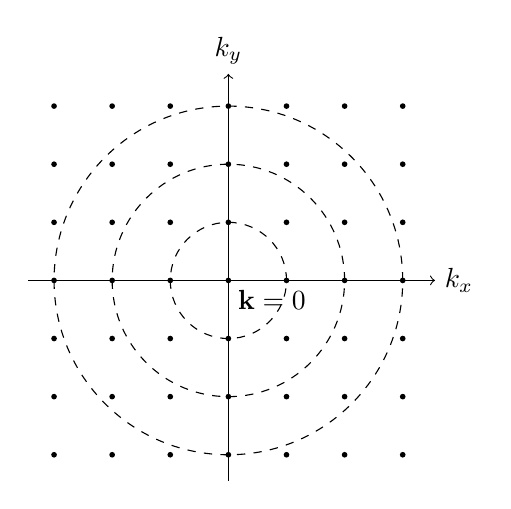
\begin{tikzpicture}[scale=0.82]
\draw[->] (-3.1,0) -- (3.2,0) node[right] {$k_x$};
\draw[->] (0,-3.1) -- (0,3.2) node[above] {$k_y$};
\draw[dashed] (0,0) circle (0.9);
\draw[dashed] (0,0) circle (1.8);
\draw[dashed] (0,0) circle (2.7);
\foreach \x in {-3,-2,-1,0,1,2,3}{
  \foreach \y in {-3,-2,-1,0,1,2,3}{
    \fill (0.9*\x,0.9*\y) circle (1.25pt);
  }
}
\node[below right] at (0,0) {$\mathbf{k}=0$};
\end{tikzpicture}
\caption{주기적 경계 조건을 적용한 유한한 상자 안 입자의 이산 운동량 상태와 일정한 에너지 껍질.}
\end{figure}

비상대론적 입자의 경우,
\begin{equation}
E_{\mathbf{k}}=\frac{\mathbf{k}^2}{2m},
\end{equation}
따라서 에너지가 가장 낮은 상태는 \(\mathbf{k}=0\)이다. 상자 안에 동일한 보손 \(N\)개를 두고 다입자 바닥 상태를 찾아보자. 첫 번째 보손은 운동량이 0인 상태에 들어간다. 두 번째 보손도 같은 상태에 들어갈 수 있고, 세 번째와 그 뒤의 모든 보손도 마찬가지다. 그러므로 보손 \(N\)개가 모두 \(\mathbf{k}=0\)를 차지한다.

이것은 보손 응축체다. 즉 동일한 입자 다수가 하나의 일입자 상태를 차지하며, 여기서는 그 상태가 최저 에너지 상태다. 운동량이 0인 파동함수는 공간적으로 일정하고 상자 전체에 걸쳐 있다. 이 파동함수는 어느 한 보손도 특정 위치에 국소화하지 않으므로, 각 보손의 위치에는 그만큼 불확정성이 있다. 점유수가 커지면 공통 파동함수의 진폭이 거시적인 장 진폭을 이루고, 장은 점점 고전적인 장처럼 거동한다.

페르미온의 바닥 상태는 이와 완전히 다르다. 우선 스핀은 무시하여 운동량 공간의 각 점이 점유 가능한 상태 하나를 나타낸다고 하자. 첫 번째 페르미온은 \(\mathbf{k}=0\)에 들어가지만, 두 번째 동일한 페르미온은 그 상태에 함께 들어갈 수 없다. 이후의 입자들은 에너지가 다음으로 낮은 껍질을 차지해야 한다. 2차원 그림에서는 에너지가 같은 가장 가까운 비영 격자점이 네 개이고, 3차원에서는 여섯 개다. 그 상태들이 점유되면 더 많은 입자는 차례로 다음 껍질들을 채워야 한다.

에너지는 운동량 공간에서 원점까지 거리의 제곱에 비례한다. 따라서 전체 에너지를 최소화하려면 배타 원리가 허용하는 범위에서 점유된 점들을 \(\mathbf{k}=0\) 주위에 최대한 가깝게 모아야 한다. 페르미온이 많으면 점유된 영역은 구에 가까워진다. 그 경계가 페르미 표면이고, 내부가 페르미 바다이며, 점유된 전체 영역을 페르미 구라고 한다. 유한한 부피에서는 허용된 점들이 격자를 이루므로 경계가 약간 울퉁불퉁하지만, 계가 크면 이 세부적인 차이는 무시할 수 있다.

\begin{figure}
\centering
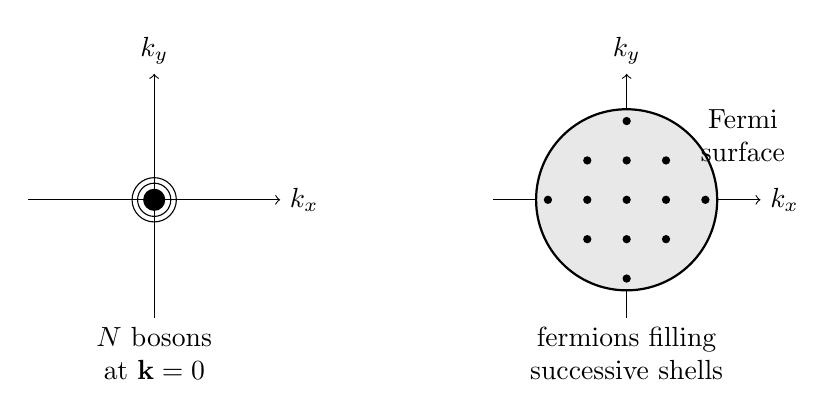
\begin{tikzpicture}[scale=1.0]
\begin{scope}[xshift=-3.0cm]
\draw[->] (-1.6,0) -- (1.6,0) node[right] {$k_x$};
\draw[->] (0,-1.5) -- (0,1.6) node[above] {$k_y$};
\fill (0,0) circle (4pt);
\draw (0,0) circle (6pt);
\draw (0,0) circle (8pt);
\node[align=center] at (0,-1.95) {$N$ bosons\\at $\mathbf{k}=0$};
\end{scope}
\begin{scope}[xshift=3.0cm]
\draw[->] (-1.7,0) -- (1.7,0) node[right] {$k_x$};
\draw[->] (0,-1.5) -- (0,1.6) node[above] {$k_y$};
\fill[gray!18] (0,0) circle (1.15);
\draw[thick] (0,0) circle (1.15);
\fill (0,0) circle (1.5pt);
\fill (0.5,0) circle (1.5pt);
\fill (-0.5,0) circle (1.5pt);
\fill (0,0.5) circle (1.5pt);
\fill (0,-0.5) circle (1.5pt);
\fill (0.5,0.5) circle (1.5pt);
\fill (0.5,-0.5) circle (1.5pt);
\fill (-0.5,0.5) circle (1.5pt);
\fill (-0.5,-0.5) circle (1.5pt);
\fill (1,0) circle (1.5pt);
\fill (-1,0) circle (1.5pt);
\fill (0,1) circle (1.5pt);
\fill (0,-1) circle (1.5pt);
\node[right,align=center] at (0.82,0.82) {Fermi\\surface};
\node[align=center] at (0,-1.95) {fermions filling\\successive shells};
\end{scope}
\end{tikzpicture}
\caption{보손은 운동량이 0인 상태에 응축하는 반면, 페르미온은 운동량 상태를 채워 페르미 표면까지 이른다.}
\end{figure}

페르미온 바닥 상태는 이에 대응하는 보손 바닥 상태보다 에너지가 훨씬 높다. 모든 보손은 운동량이 영인 상태에 머물 수 있지만, 페르미온 대부분은 운동량이 영이 아닌 상태에 놓일 수밖에 없다. 페르미온을 더 추가할수록 점유된 운동량의 최댓값이 커진다. 게다가 큰 운동량의 껍질에는 원점 근처의 껍질보다 격자점이 더 많다. 따라서 큰 페르미 구에는 상당한 운동량을 가진 입자가 많이 들어 있고, 가장 낮은 운동량 상태에 있는 입자는 소수뿐이다.

들뜬 상태에서도 차이는 이어진다. 보손의 첫 번째 들뜬 상태는 응축체에서 보손 하나를 꺼내 첫 번째 들뜬 일입자 상태에 놓아 만들 수 있다.
\begin{equation}
(N,0,0,\ldots)\longrightarrow (N-1,1,0,\ldots).
\end{equation}
어느 보손을 옮기는지는 중요하지 않다. 입자들이 서로 동일하기 때문이다. 더 높은 들뜬 상태는 여러 방식으로 만들 수 있다. 준위 간격에 따라 보손 하나를 더 높은 준위에 놓거나, 보손 두 개를 첫 번째 들뜬 준위에 놓을 수 있다. 보손계를 들뜨게 한다는 것은 입자들을 응축체에서 더 높은 에너지 상태로 올리는 것이다.

페르미온의 경우, 채워진 페르미 구 안의 다른 점으로 입자를 옮길 수 없다. 그 점들이 이미 모두 점유되어 있기 때문이다. 페르미 바다 깊은 곳에서 페르미온 하나를 꺼내 표면 위에 놓는 것은 가능하지만, 큰 에너지가 든다. 에너지 비용이 가장 적은 들뜸은 페르미 표면 바로 안쪽에서 페르미온 하나를 꺼내 표면 바로 바깥의 비점유 상태로 옮기는 것이다. 올라간 전자는 표면보다 에너지가 조금 높고, 비어 있게 된 상태는 표면보다 에너지가 조금 낮다.

\begin{figure}
\centering
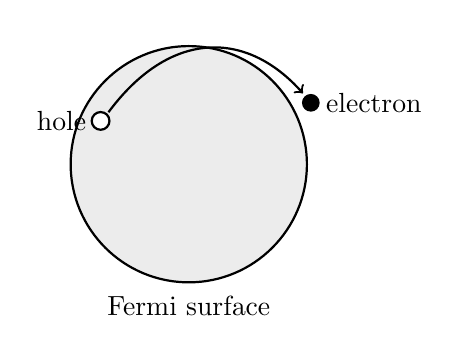
\begin{tikzpicture}[scale=1.0]
\fill[gray!15] (0,0) circle (1.5);
\draw[thick] (0,0) circle (1.5);
\draw[fill=white,thick] (-1.12,0.55) circle (3.2pt);
\fill (1.55,0.78) circle (3.2pt);
\draw[->,thick] (-1.02,0.66) .. controls (-0.25,1.7) and (0.72,1.72) .. (1.45,0.9);
\node[left] at (-1.18,0.55) {hole};
\node[right] at (1.62,0.78) {electron};
\node[below] at (0,-1.55) {Fermi surface};
\end{tikzpicture}
\caption{저에너지 페르미온 들뜸에서는 전자가 페르미 표면을 가로질러 올라가며 그 자리에 정공이 남는다.}
\end{figure}

\section{정공과 저에너지 들뜸}

정공의 전하를 구체적으로 생각해 보기 위해 상자의 부피 전체에 양전하가 균일하게 퍼져 있다고 하자. 실제 물질에서 이 양전하는 궁극적으로 원자핵 속 양성자에서 오지만, 균일하게 분포한다고 두면 모형이 간단해진다. 이 배경 전하를 중화할 만큼 전자를 더한다. 바닥 상태에서는 전자들이 페르미 구를 채운다.

전자 하나를 페르미 표면 아래에서 위로 올려도 상자의 전체 전하는 변하지 않는다. 이 과정에서 표면 위에는 음전하를 띤 전자가 생기고, 표면 아래에는 음전하가 빠진 자리가 남는다. 그러므로 빠진 전자는 양전하를 띤 들뜸, 즉 정공으로 취급할 수 있다.

\begin{classroomqa}
\lecturetimestamp{01:31:38}
\audiencequestion{페르미 표면 아래의 정공은 음의 에너지를 갖나요?}
\lecturerresponse{아닙니다. 정공은 다체 바닥 상태보다 높은 들뜬 상태이므로 들뜸 에너지는 양수입니다. 페르미 표면을 기준으로 에너지를 재면, 점유된 전자를 표면 아래에서 제거하는 데 양의 에너지가 듭니다.}
\end{classroomqa}

제거된 전자의 에너지를 \(\varepsilon<\varepsilon_F\)라 하고, 위로 올라간 전자의 에너지를 \(\varepsilon'>\varepsilon_F\)이라 하자. 공급된 에너지는 페르미 표면으로부터의 양의 거리 두 개로 나누어 쓸 수 있다.\footnote{두 구간은 각각 따로 제시되어 있다. 여기 보인 간결한 등식은 이를 대수적으로 동등한 형태로 다시 쓴 것이다.}
\begin{equation}
\Delta E
=\varepsilon'-\varepsilon
=(\varepsilon'-\varepsilon_F)+(\varepsilon_F-\varepsilon).
\end{equation}
첫 번째 항은 페르미 표면 위 전자의 에너지로, 두 번째 항은 그 아래 정공의 에너지로 보는 것이 자연스럽다.
\begin{equation}
E_{\mathrm{electron}}=\varepsilon'-\varepsilon_F>0,
\qquad
E_{\mathrm{hole}}=\varepsilon_F-\varepsilon>0.
\end{equation}
전자는 음전하를 띠고 정공은 양전하를 띤다.

페르미 표면 위의 전자는 나중에 빈 정공 자리에 내려올 수 있다. 이때 전자의 에너지가 낮아지므로 방출된 에너지는 복사로 빠져나가야 한다. 전자가 점유되지 않은 낮은 상태로 내려오면서 광자 하나 이상을 방출한다고 설명할 수 있다. 또는 전자와 정공이 소멸하여 복사가 된다고 말할 수도 있다. 정공은 상자의 기본 구성 성분이 추가된 것이 아니라, 전자로 채워진 상태에 생긴 빈자리다. 그렇더라도 정공의 에너지와 전하를 고려하면 입자 같은 들뜸으로 취급하는 것이 유용하다.

\begin{classroomqa}
\lecturetimestamp{01:36:52}
\audiencequestion{전자를 들뜬다는 것은 운동량 공간의 격자점 하나에서 다른 격자점으로 옮긴다는 뜻인가요?}
\lecturerresponse{전자를 한 에너지 준위에서 다른 에너지 준위로 옮긴다는 뜻입니다. 상자 속 자유 입자에서는 운동량 격자가 그 준위들을 표시하지만, 이 개념이 운동량 공간의 격자에 의존하는 것은 아닙니다. 원자에서는 양전하가 원자핵에 집중되어 있습니다. 전자들은 가능한 원자 준위 중 가장 낮은 것부터 채우며, 광자는 전자 하나를 들뜬 준위로 올려 보낼 수 있습니다. 그러면 전자가 있던 준위에 빈자리가 남습니다. 이 빈자리가 원자에서 정공에 해당합니다.}
\end{classroomqa}

상자에서도 광자 흡수는 광자의 에너지를 페르미 표면 위의 전자와 표면 아래의 정공으로 바꾼다. 원자에서는 같은 표현으로 들뜬 전자와 점유된 낮은 준위에 남은 빈자리를 함께 묘사한다.

\begin{classroomqa}
\lecturetimestamp{01:39:16}
\audiencequestion{저에너지 광자가 페르미 구 안의 어디에 있는 전자든 흡수될 수 있나요?}
\lecturerresponse{아닙니다. 전자가 페르미 바다 깊은 곳에 있으면 주변 상태가 모두 이미 점유되어 있고, 저에너지 광자로는 표면 위의 비점유 상태까지 전자를 올릴 수 없습니다. 광자가 가진 에너지 범위 안에 접근 가능한 빈 상태가 있는 전자는 페르미 표면에 충분히 가까운 경우뿐입니다. 충분히 에너지가 큰 광자는 페르미 바다 깊은 곳의 전자도 들뜨게 할 수 있습니다.}
\end{classroomqa}

따라서 저에너지 흡수 단면적은 페르미 바다 전체 부피가 아니라 그 표면에 의해 좌우된다. 페르미 바다 깊은 곳의 전자는 작은 전이를 일으킬 수 없도록 막혀 있지만, 표면 바로 아래의 전자는 바로 위로 올라갈 수 있다.

\begin{classroomqa}
\lecturetimestamp{01:40:42}
\audiencequestion{입사 광자 없이 전자끼리 직접 상호작용하는 것을 막는 것은 무엇인가요?}
\lecturerresponse{아무것도 없습니다. 이 단순한 모형에서는 전자--전자 상호작용을 무시하고 있습니다. 이를 포함하면 페르미 바다 그림이 더 복잡해지기 때문입니다. 금속을 다루는 첫 번째 근사에서는 전자들의 유효한 영향이 대체로 무시해도 될 만큼 약하다고 봅니다.}
\end{classroomqa}

\begin{classroomqa}
\lecturetimestamp{01:41:10}
\audiencequestion{광자 하나가 전자 여러 개를 들뜨게 할 만큼 충분한 에너지를 지니면 어떻게 되나요?}
\lecturerresponse{보존 법칙에 부합하는 과정은 원칙적으로 무엇이든 가능합니다. 광자는 전자--정공 쌍을 둘 이상 만들 수 있습니다. 전자 두 개를 들뜨게 하면 정공도 두 개 남습니다. 이런 과정은 들뜸을 더 많이 만들며, 그 에너지로 전자 하나를 훨씬 강하게 들뜨게 하는 경우보다 일반적으로 확률이 낮습니다.}
\end{classroomqa}

\begin{classroomqa}
\lecturetimestamp{01:42:06}
\audiencequestion{광자 하나만으로는 들뜸을 만들 수 없을 때 광자 두 개가 함께 흡수될 수 있나요?}
\lecturerresponse{네. 흡수는 확률적인 과정입니다. 광자 각각의 에너지는 필요한 에너지보다 낮더라도 두 광자의 에너지 합이 가능한 들뜸에 도달하면 2광자 과정이 일어날 수 있습니다. 주어진 빛의 에너지로 허용된 들뜸에 도달할 수 없다면, 빛은 대부분 계를 그대로 통과합니다.}
\end{classroomqa}

\editorialnote{이 부분의 짧은 논의는 흡수된 복사를 전자의 집단 운동과 연결하지만, 구체적인 내용은 복원할 수 없다. 확실한 것은 이러한 집단 응답이 단일 입자--정공 그림보다 더 복잡하다는 진술뿐이다.}

\begin{classroomqa}
\lecturetimestamp{01:43:49}
\audiencequestion{모든 전자가 같은 음전하를 띠는데 전자--전자 상호작용을 약하다고 하는 이유는 무엇인가요?}
\lecturerresponse{전자들은 이를 상쇄하는 양전하 배경 속에 놓여 있습니다. 이 배경은 전자의 전하를 차폐하여 이 단순화된 상황에서 유효 상호작용을 줄입니다. 상호작용이 사라지는 것은 아닙니다. 이를 다루려면 매질의 차폐 응답을 고려해야 합니다.}
\end{classroomqa}

\begin{classroomqa}
\lecturetimestamp{01:44:41}
\audiencequestion{차폐는 나중에 다루나요?}
\lecturerresponse{네. 차폐는 중요하지만, 상호작용하는 계를 더 온전히 다룰 수 있을 때까지 미룹니다.}
\end{classroomqa}

\section{1차원 페르미온 바다와 반입자}

정공을 도입하는 구성은 반입자 개념으로 이어진다. 물질 속 전자에 적용한 것과 같은 논리 구조를 상대론적 양자장과 그 진공에도 적용할 수 있다. 가장 단순한 경우로 공간 차원이 하나인 질량 없는 페르미온 장 \(\psi(x,t)\)을 생각하자. 빛의 속도를 1로 둔 단위계에서 가능한 두 선형 분산 관계는 다음과 같다.
\begin{equation}
\omega=k,
\qquad\text{or}\qquad
\omega=-k.
\end{equation}
여기서는 첫 번째 가지를 구체적으로 살펴본다.

\editorialnote{마지막 문답에서는 서로 양립할 수 없는 입자 식별 방식이 번갈아 등장한다. 확실한 모형은 한 공간 차원에서 한 방향으로만 전파되는, 정체가 특정되지 않은 질량 없는 페르미온 장을 다루는 장난감 모형이다.}

평면파
\begin{equation}
\psi(x,t)=e^{i(kx-\omega t)},
\end{equation}
의 경우 미분은 다음과 같다.
\begin{equation}
\frac{\partial\psi}{\partial t}=-i\omega\psi,
\qquad
\frac{\partial\psi}{\partial x}=ik\psi.
\end{equation}
따라서 \(\omega=k\)이면 다음의 1계 장 방정식이 성립한다.
\begin{equation}
\frac{\partial\psi}{\partial t}
=-\frac{\partial\psi}{\partial x}.
\end{equation}

\begin{figure}
\centering
\includegraphics[width=0.72\textwidth]{lecture_05_figure_05.png}
\caption{평면파가 \(\omega=k\)를 만족하는 1계 장 방정식을 도입한다.}
\lectureframe{01:47:22}
\end{figure}

\(f(x-t)\) 형태의 임의의 프로필은 이 방정식을 만족하며 오른쪽으로 이동한다. 부호를 반대로 하면 다음을 얻는다.
\begin{equation}
\frac{\partial\psi}{\partial t}
=+\frac{\partial\psi}{\partial x},
\end{equation}
이때 프로필 \(f(x+t)\)은 왼쪽으로 이동한다. 각 1계 방정식은 운동 방향 하나만을 선택한다. 장은 페르미온 장이라고 하자. 정공 논의를 위해 장의 입자들이 전하를 띤다고 가정하자.

가지 \(\omega=k\)에는 곧바로 어려움이 드러난다. 파수 \(k\)는 음수일 수 있고, 따라서 \(\omega\)도 음수일 수 있다. \(\omega\)가 이 단위계에서 에너지이므로, 직선형 스펙트럼에는 양의 에너지 상태와 음의 에너지 상태가 모두 포함된다.
\begin{equation}
E=\omega=k.
\end{equation}

\begin{figure}
\centering
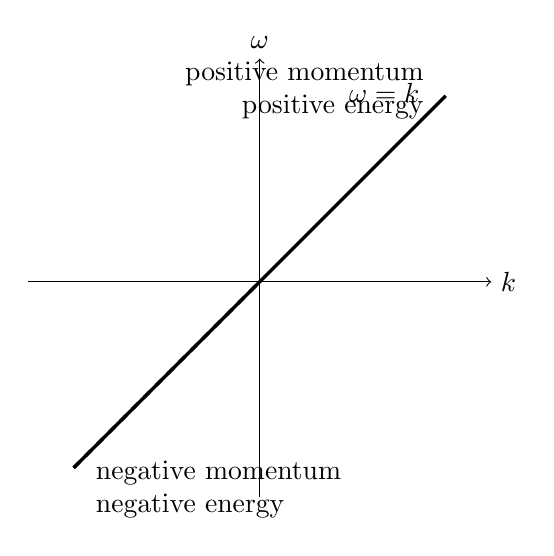
\begin{tikzpicture}[scale=1.05]
\draw[->] (-2.8,0) -- (2.8,0) node[right] {$k$};
\draw[->] (0,-2.6) -- (0,2.7) node[above] {$\omega$};
\draw[very thick] (-2.25,-2.25) -- (2.25,2.25);
\draw[very thick,dashed] (-2.25,-2.25) -- (0,0);
\node[above left] at (2.05,2.05) {$\omega=k$};
\node[below right,align=left] at (-2.1,-2.05) {negative momentum\\negative energy};
\node[above left,align=right] at (2.1,1.85) {positive momentum\\positive energy};
\end{tikzpicture}
\caption{음의 에너지 절반이 \(k<0\)에 있는 단일 가지 스펙트럼 \(\omega=k\).}
\end{figure}

보통의 빈 진공은 이런 이론의 바닥 상태가 될 수 없다. 양의 에너지를 가진 페르미온은 광자를 방출하고 더 낮은 상태로 내려갈 수 있다. 에너지가 0인 곳에서 멈추게 할 것은 없다. 음의 에너지 상태로 계속 내려가면서 더 많은 복사를 방출하고 끝없이 추락할 수 있다. 페르미온이 잃은 에너지는 복사장에 나타난다. 따라서 아래로 한없이 이어지는 스펙트럼에서는 안정된 보통의 진공을 얻을 수 없다.

페르미온의 배타 원리를 이용하면 다른 출발점을 얻는다. 음의 에너지인 일입자 상태를 모두 0에 이르기까지 페르미온 하나씩 채운다. 각 상태가 이미 점유되어 있으므로 다른 페르미온은 그 상태들로 더 내려갈 수 없다. 음의 에너지 페르미온을 더 넣는 것은 불가능하고, 양의 에너지 페르미온을 넣으면 에너지가 증가한다. 따라서 음의 에너지 상태를 완전히 채운 바다를 다체 바닥 상태로 삼을 수 있으며, 이를 진공이라고 부른다.

\begin{figure}
\centering
\resizebox{\linewidth}{!}{%
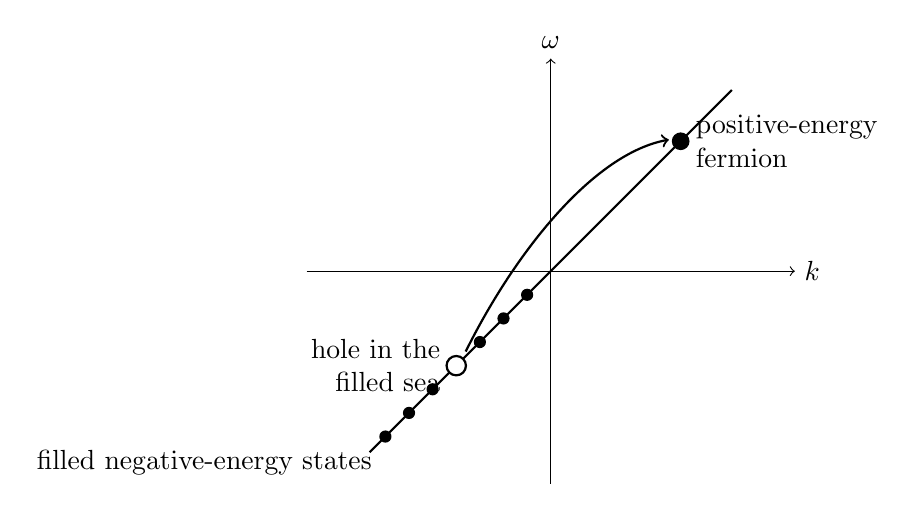
\begin{tikzpicture}[scale=1.0]
\draw[->] (-3.1,0) -- (3.1,0) node[right] {$k$};
\draw[->] (0,-2.7) -- (0,2.7) node[above] {$\omega$};
\draw[thick] (-2.3,-2.3) -- (2.3,2.3);
\foreach \p in {-2.1,-1.8,-1.5,-1.2,-0.9,-0.6,-0.3}{
  \fill (\p,\p) circle (2.2pt);
}
\draw[fill=white,thick] (-1.2,-1.2) circle (3.5pt);
\fill (1.65,1.65) circle (3.2pt);
\draw[->,thick] (-1.08,-1.02) .. controls (-0.45,0.25) and (0.55,1.5) .. (1.5,1.67);
\node[left,align=right] at (-1.28,-1.2) {hole in the\\filled sea};
\node[right,align=left] at (1.72,1.65) {positive-energy\\fermion};
\node[below left] at (-2.15,-2.15) {filled negative-energy states};
\end{tikzpicture}%
}
\caption{음의 에너지 상태를 채운 바다와 페르미온 하나를 양의 에너지 상태로 올려 만든 들뜸.}
\end{figure}

가장 단순한 들뜸은 음의 에너지 바다에서 페르미온 하나를 꺼내 양의 에너지 상태에 놓는 것이다. 올라간 페르미온은 보통의 양의 에너지 입자다. 바다에 남은 빈자리는 두 번째 들뜸인 정공이다. 제거된 페르미온이 음전하를 띠었다면 정공은 양전하를 띤다.

이 한 가지 예에서 정공은 양의 운동량도 갖는다. 빠진 페르미온이 운동량 \(k_-<0\)인 상태를 차지했다면, 이를 제거함으로써 전체 운동량은 다음만큼 변한다.
\begin{equation}
p_{\mathrm{hole}}=-k_->0.
\end{equation}
이는 음의 운동량이 부족해진 것이다. 따라서 들뜸은 양의 에너지와 음전하를 가진 페르미온, 그리고 양의 에너지와 양전하를 가진 정공으로 이루어진다. 두 들뜸 모두 양의 운동량을 가지며, \(\omega=k\) 가지에서는 오른쪽으로 움직인다.

완전한 전자 이론에서 양전하를 띤 정공은 양전자다. 디랙은 처음에 정공을 양성자와 동일시하는 방안을 고려했다. 이 구성에서는 입자와 그 반입자의 질량이 같아야 한다. 정공은 전자와 질량이 같고 전기적 전하가 반대인 별개의 입자다. 이것이 음의 에너지 스펙트럼으로부터 나온 기본적인 입자--반입자 해석이다.

같은 방식으로 보손을 다룰 수는 없다. 보손 상태에는 입자를 얼마든지 넣을 수 있으므로, 음의 에너지 준위를 한 번 채워 더 이상의 점유를 막을 방법이 없다. 보손을 그 준위에 더 넣을 때마다 에너지는 계속 낮아질 수 있다.
\begin{equation}
\begin{aligned}
\text{fermionic mode: }&n=0\ \text{or}\ 1,\\
\text{bosonic mode: }&n=0,1,2,\ldots .
\end{aligned}
\end{equation}
따라서 제안된 보손 계에는 여전히 바닥 상태가 없다. 이 기초적인 구성에서 채워진 바다의 안정성은 정확히 페르미온의 배타 원리에 달려 있다.

이 1차원 방정식은 디랙 방정식의 장난감 모형일 뿐이다. 이 장은 질량이 없고 빛의 속도로 움직이며 한 방향으로만 전파된다. 더 완전한 디랙 방정식은 빠져 있는 운동 방향과 상대론적 입자 구조의 나머지 요소를 포함해야 한다. 보손 장의 반입자 처리와 함께 그 완전한 방정식은 뒤로 미룬다.
